\section{Modeling and Analysing a Architecture for Video Streaming Provisioning}
\label{sec:system-archi}

%{\color{blue} This section explains the architecture system, and what it is  for, explaining some protocols flowcharts. Studying the protocols and focusing in the system part of the experiments.}

This section explains the modeling used in our experiments. We first provide an overview of the proposed video streaming service architecture using Controller-assisted and SVC including its rationale. The remaining subsections describe the implementation of this service architecture.

\subsection{Impact of Fog Multi-tier Network Approach}

A vertically edge architecture with N levels aims to: \textit{i)} Improve the QoE of users, serving the requested content as close to the user as possible; \textit{ii)} Reduce congestion at the core of the network; \textit{iii)} efficiently deal with the amount of data that needs to be processed and extract meaningful data to create more intelligence at each level.

To confirm these diference in users performance requesting a video from a node in different tiers, . We present two users requesting requesting a multimedia content in different layers on the network to address the impact occurred. In Figure~\ref{fig:impact-two-layers}, the graphs show the results of bitrate, interruptions, buffer and representations switch, respectively from left to the right, and along x-axis the simulation time. 

As we can see, both users have had no interruptions throughout the video, besides the initial interruption until the start of the video. However, the user who received the video on the nearest fog layer had a higher bit rate than the other user. As well as the buffer was soon filled and the user had the best possible resolution of the video. Whereas the user who received the video from a more distant layer, in some moments, worked with the buffer at the limit and had to constantly switch resolutions so that there is no interruption during the video execution.



\begin{figure}
    \centering
    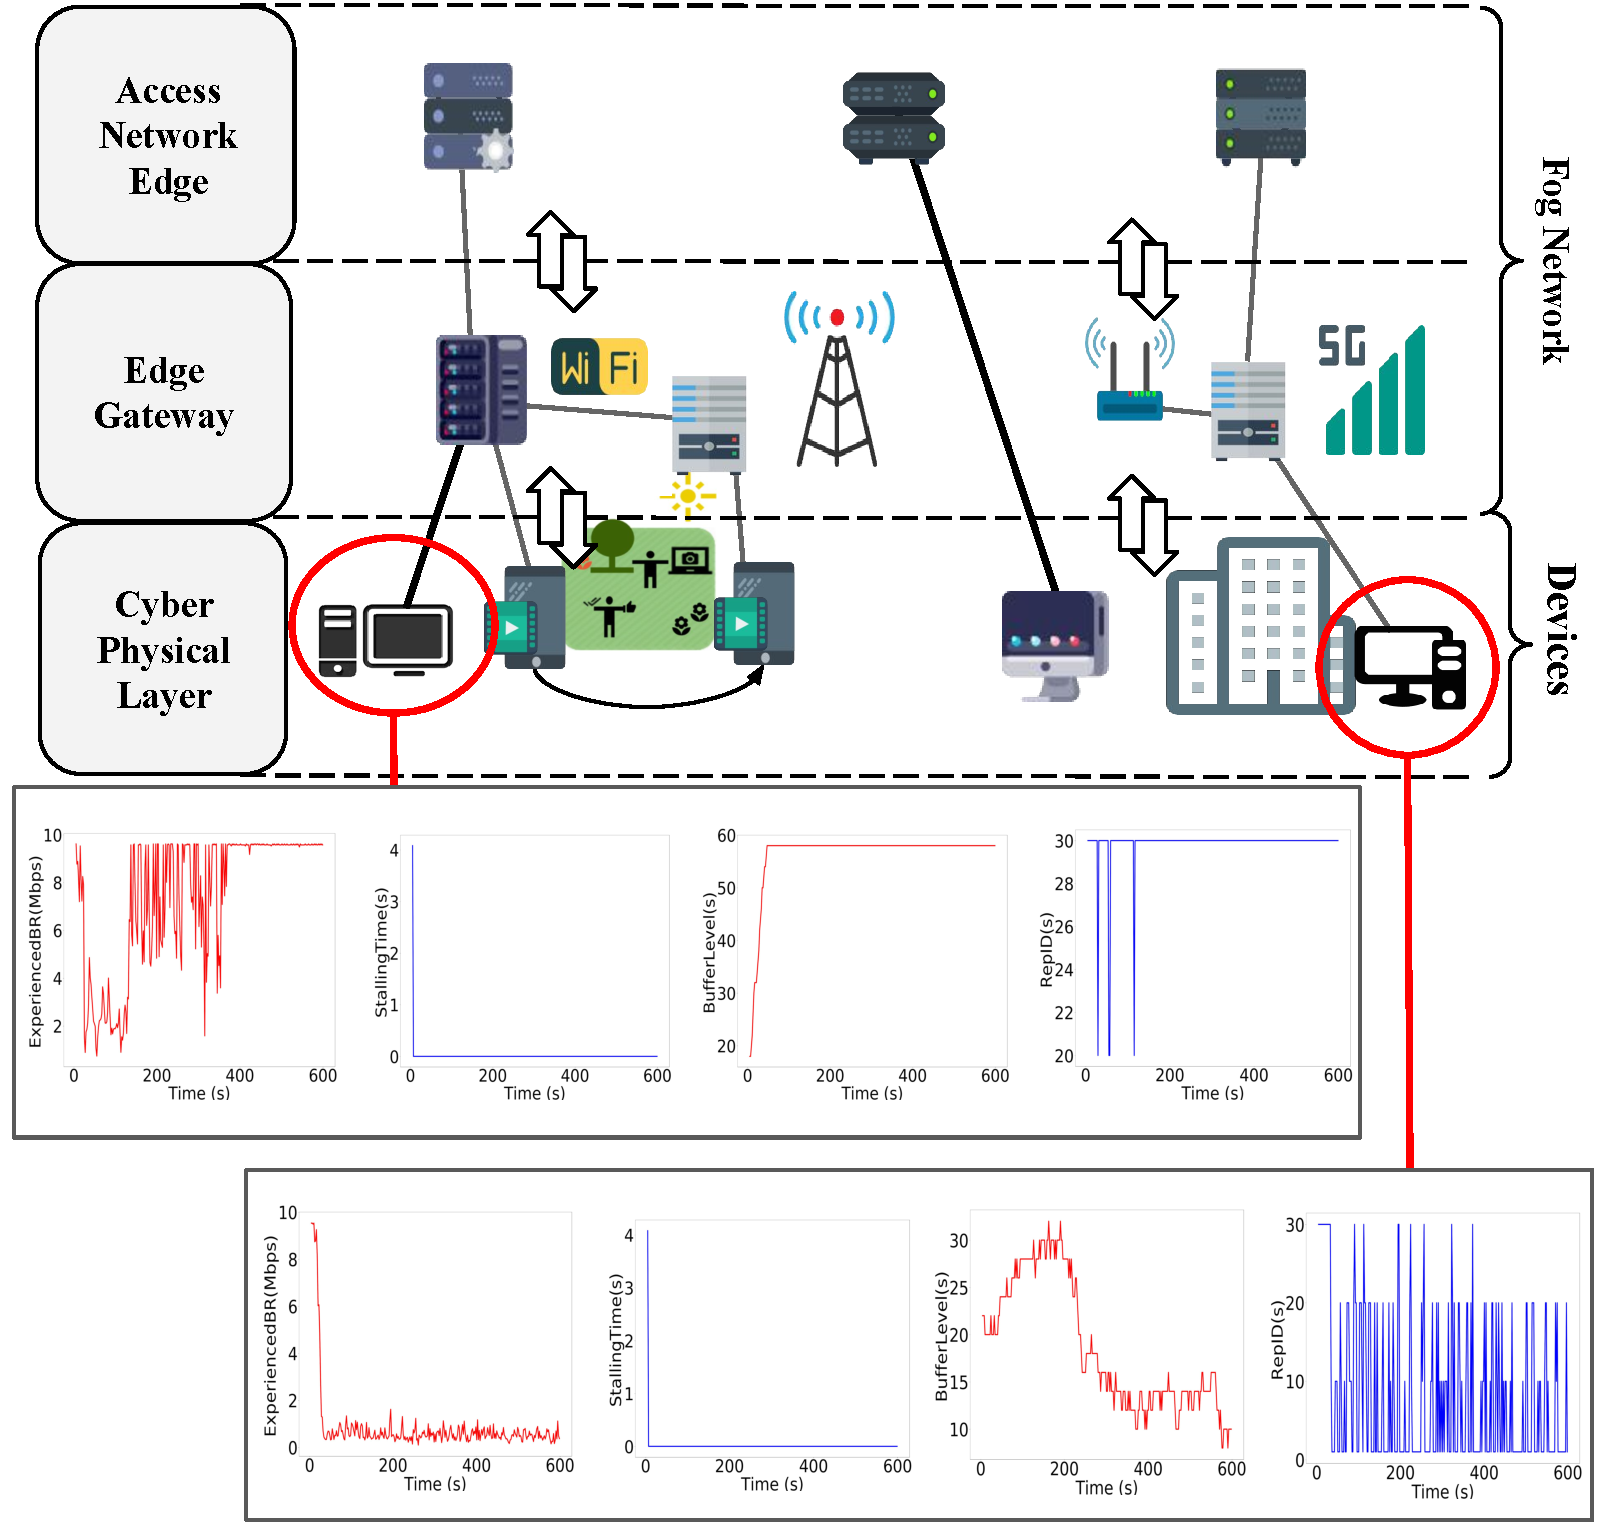
\includegraphics[width=0.9\linewidth]{images/qoe-multi-level.pdf}
    \caption{\textbf{The number of bitrate switches, stalls, buffer size, the startup delay in seconds of a DASH player requesting a video with 10 bitrate levels varying from 50 to 4,500Kbps and from nodes in different tiers.}}
    \label{fig:impact-two-layers}
\end{figure}


\subsection{Multi-tier Edge-Cloud Network Opportunities}

Esta seção apresenta algumas oportunidades dentro de redes multi-tier edge/cloud para o provisionamento da transmissção de videos. Aproveitar nós próximos aos usuários podem melhorar o funcionamento do rede como um todo, aqui nós discutimos alguns insights que podem ser usados em favor dos stakeholders que utilizam a infraestrutura para transmissão de video. 


\subsubsection{Improving User QoE}

The results reported in Fig~\ref{fig:impact-two-layers} shows that a edge multi-tier network improves the users' QoE, serving the requested content as close to the user as possible. 

\subsubsection{Potential Bandwith Saving}



\subsubsection{Cacheability}


Caching audio/video during peak hours ...


\subsection{Resource Requirements based on QoS}

Manage the QoE users refer to those service where the satisfaction guarantees can be centrally controlled by the controller. The Controller can address this problem by creating a control channel to managed-quality video streaming services over the edge-cloud network.
%l